\documentclass{article}
\usepackage{../../Self_Style}

\title{Phys 20AL Lab Report Week 2: Friction}
\author{Zih-Yu Hsieh}
\date{\today}

\begin{document}
\maketitle

\tableofcontents

\pagebreak 

\section{Introduction and Goal of the Experiment}
Friction is an observed action between two objects when their surfaces have nontrivial collision, which provides a force in the opposite direction of each object's traveling direction.

Physicists have observed that when an object is static on a surface, the force required to set the object in motion in most cases are explicitly larger compared to the force required to keep an object in motion, which indicates that the friction under static and moving scenrios could be different.

Another observation that has been made is the proportionality of friction together with the normal force of the surface: Given the force applied by the surface on the object, that is orthogonal to the given surface, the normal force measured friction fore are proportional, which the constant of proportionality is named as \emph{Coefficient of Static / Kinetic Friction} depending on the scenarios.

\hfil

Given a ramp with angle $\theta$, an object with mass $m$, and the coefficient of friction (depending on the scenario), the current model for friction provides the static friction $F_f$ as follow:
\begin{figure}[h!]
    \centering
    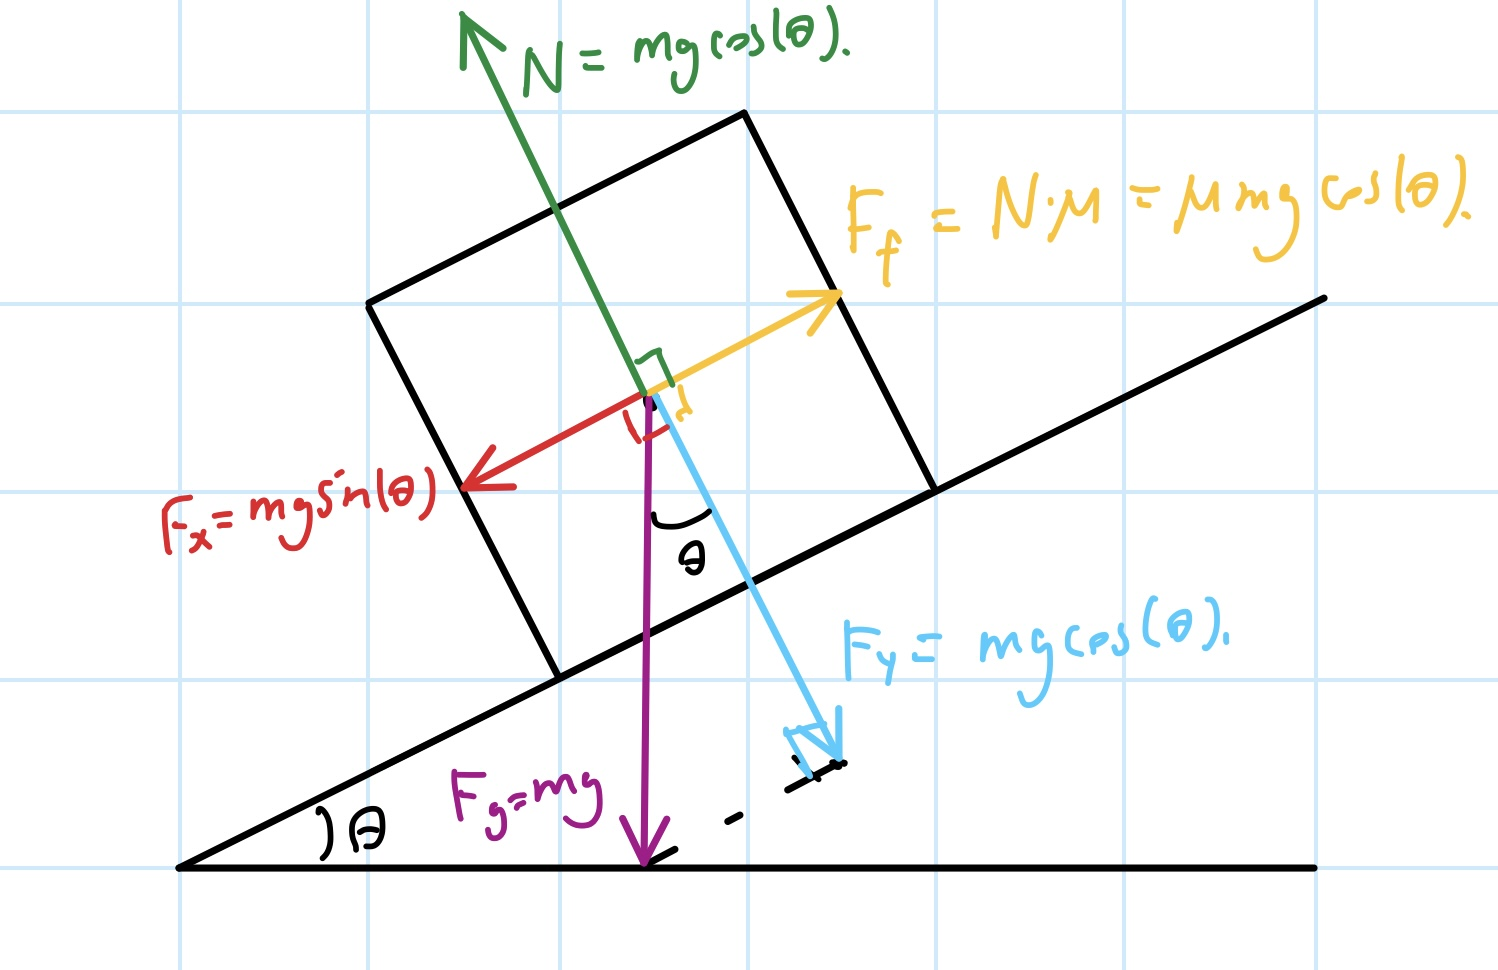
\includegraphics[width=100mm]{friction_explain.jpg}
    \caption{The Diagram of Friction of an Object on a Ramp}
    \label{graph:friction-diagram}
\end{figure}
Which, with the object stays in stationary, $F_f=F_x$ in terms of their magnitude, showing that the coefficient of static friction $\mu = \frac{F_f}{N}=\frac{mg\sin(\theta)}{mg\cos(\theta)} = \tan(\theta)$.

For kinetic energy, it's instead calculating the friction force $F_f$ as a whole, and calculate the coefficient of kinetic friction as $\mu=\frac{F_f}{N}$.

\hfil

With such model and some basics of friction in mind, the aim of this experiment includes:
\begin{itemize}
    \item Observe the relationship between the material of the surface and mass of the object with static friction, and calculate the coefficient of static friction.
    \item Calculate the coefficient of kinetic friction when fixing surface material and mass of the object.
    \item Check the uncertainty of the observed friction from the model's prediction.
\end{itemize}

\pagebreak

\section{Experimental Setup}
The equipments for this experiment include: meter stick, tape, masses, mass scale, stand, wooden ramp, clamp, different surface materials for the ramp (this experiment specifically uses paper and plastic board), protractor, and a cart.

\hfil

The setup of the experiment goes as follow:
\begin{itemize}
    \item[1.] Fix the stand next to the table.
    \item[2.] Fix the clip onto the wooden ramp, clamp the clip onto the stand, and let one side of the wooden ramp lay on the table. This is used for adjusting the angle of the ramp.
    \item[3.] Fix the protractor's center at the edge of the wooden ramp that's touching the table, which is used to measure the angle.
    \item[4.] Tape the (desired) surface for the experiment (ex: plastic board, paper, etc.) onto the wooden ramp.
\end{itemize}

\begin{figure}[h!]
    \centering
    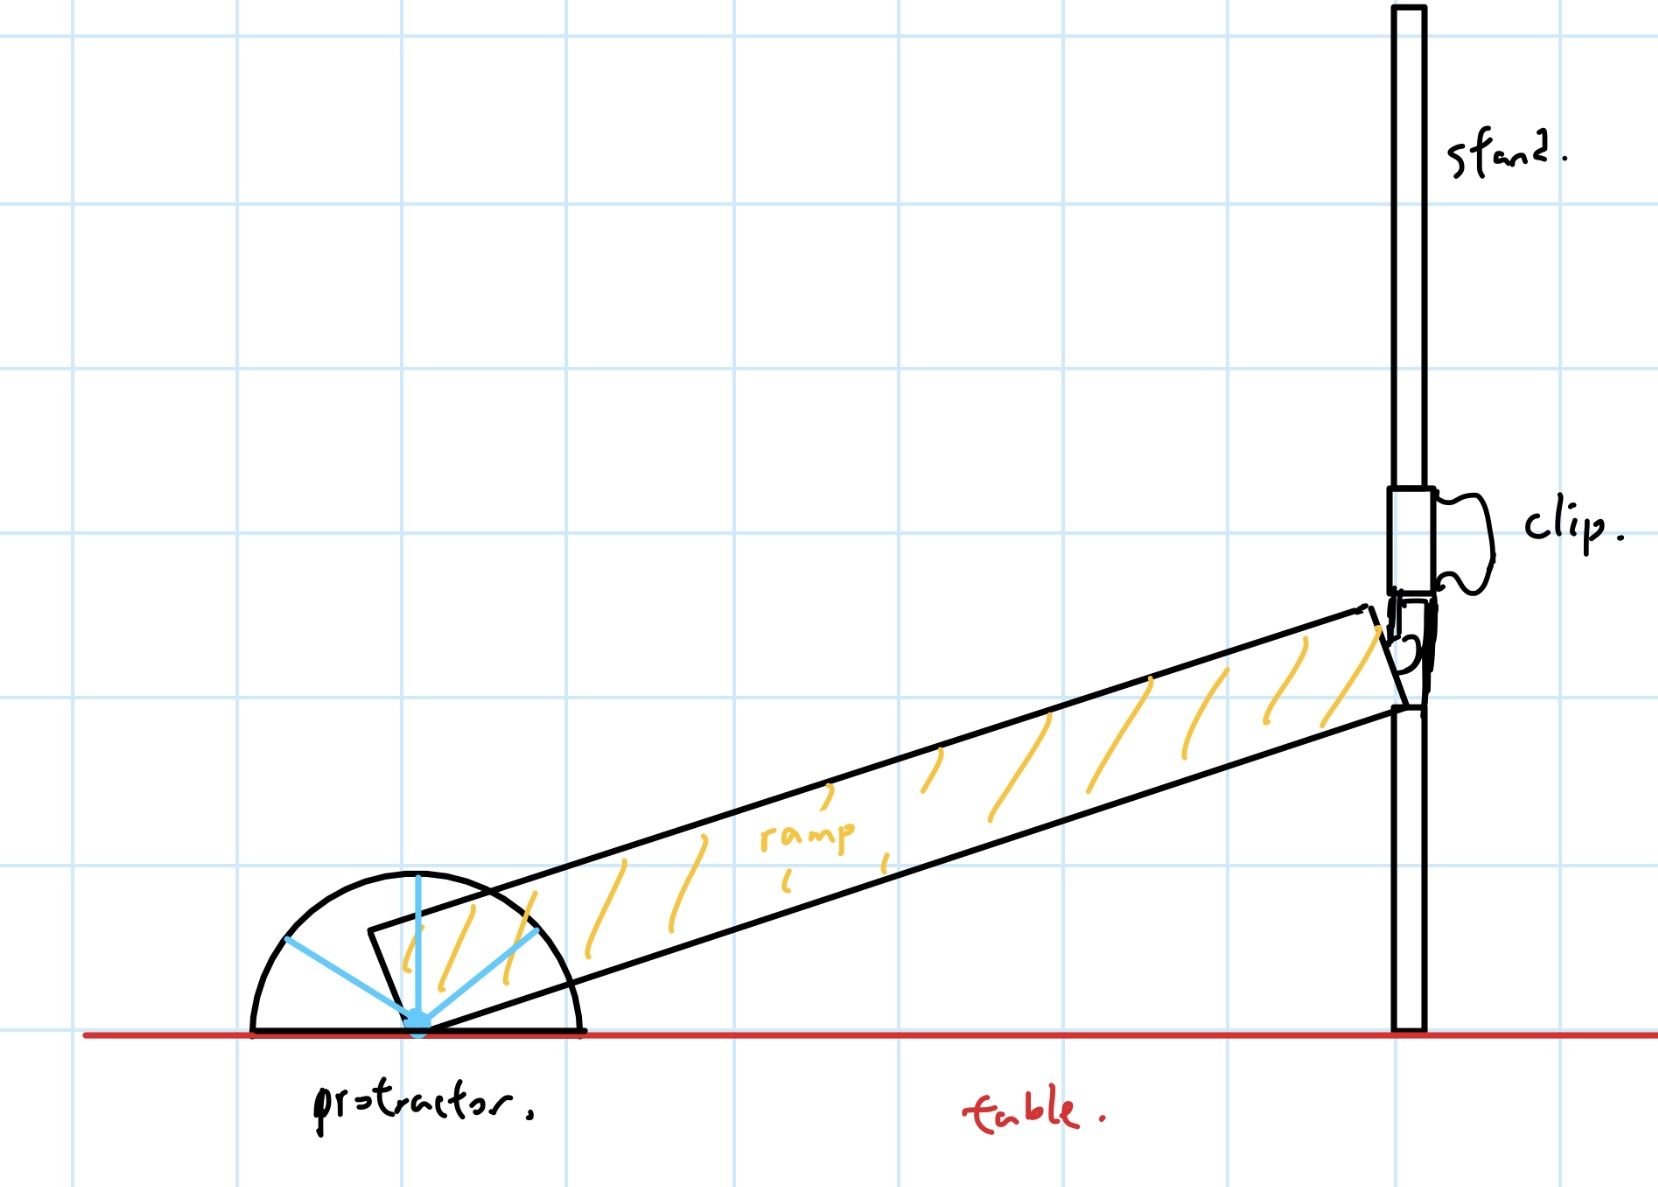
\includegraphics[width=100mm]{setup_sketch.jpg}
    \caption{Sketch of the Experimental Setup}
    \label{fig:sketch_setup}
\end{figure}

%resolve this issue with the other computer
\begin{comment} 
\begin{figure}[h!]
    \centering
    \begin{subfigure}[t]{0.3\textwidth}
        \centering
        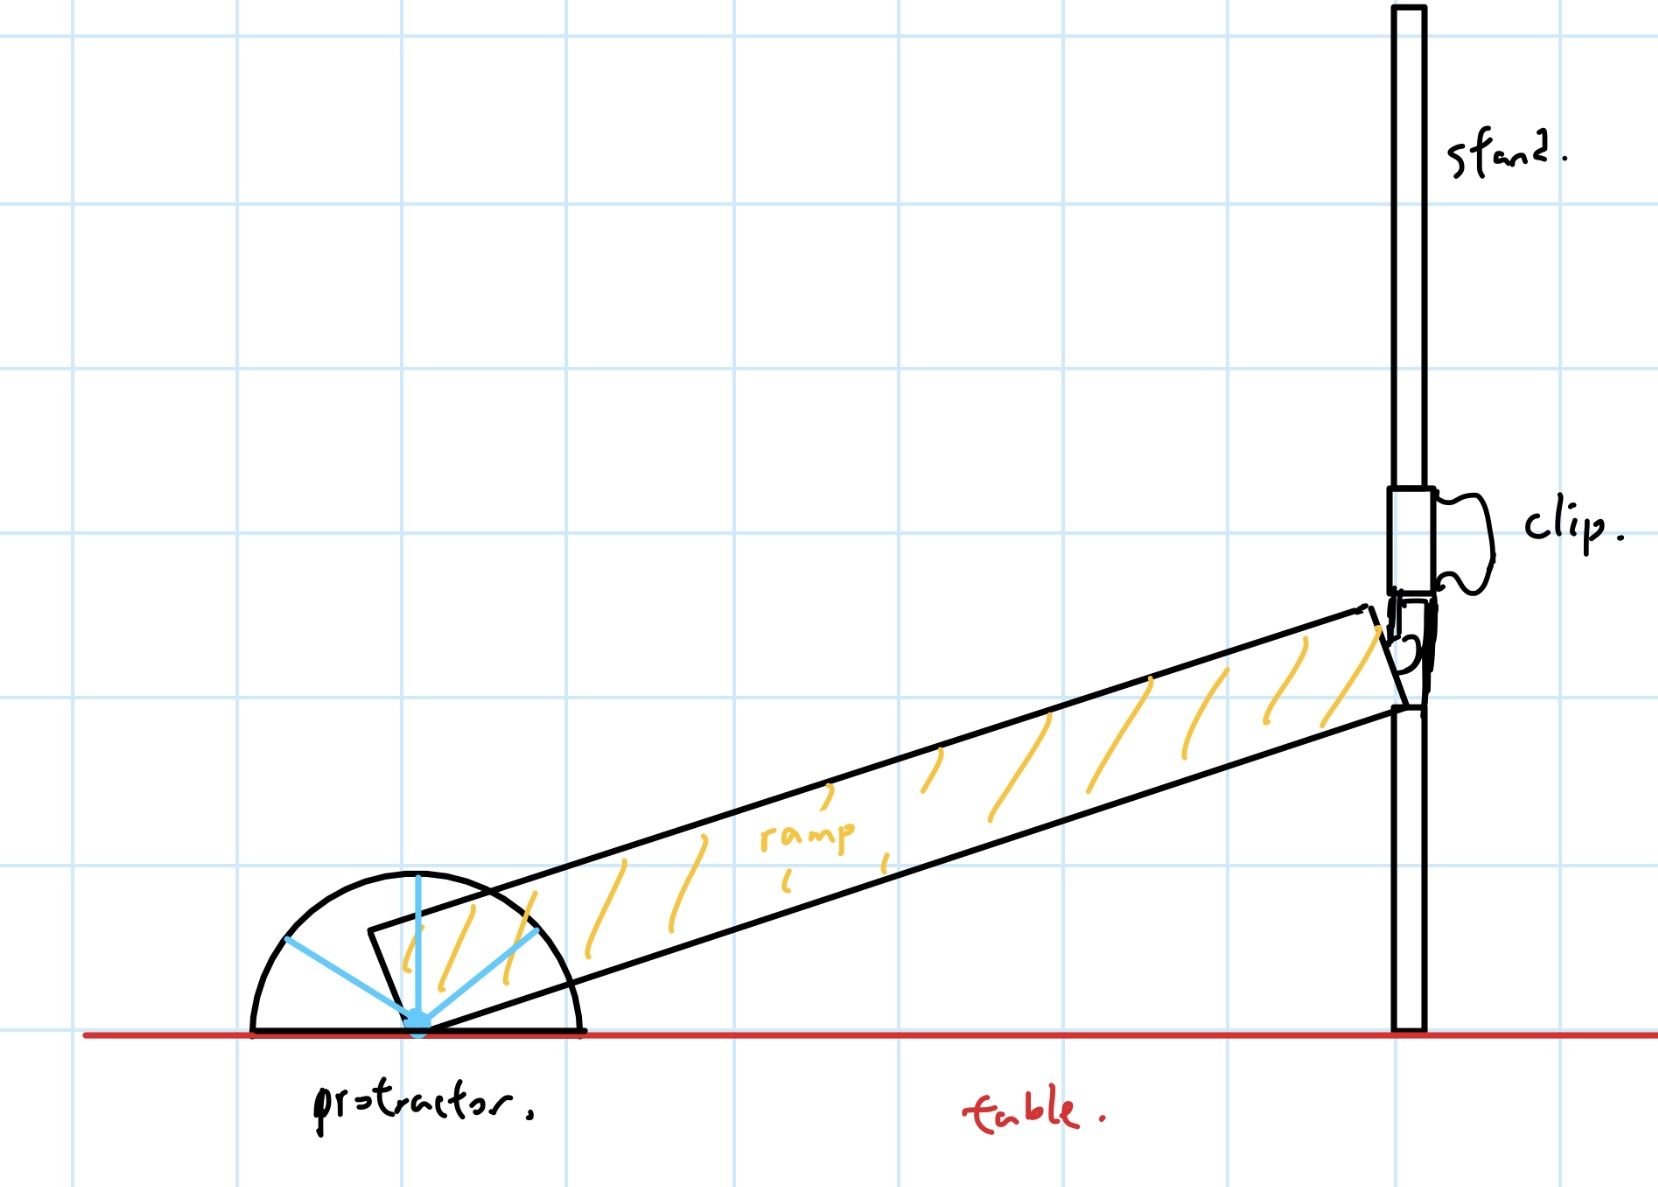
\includegraphics[width=100mm]{setup_sketch.jpg}
        \caption{Sketch of the Experimental Setup}
        \label{fig:sketch_setup}
    \end{subfigure}%
    \hfil 
    \begin{subfigure}[t]{0.2\textwidth}
        \centering
        \includegraphics[width=\linewidth]{lab_setup2.jpg}
        \caption{Photo of the Equipment Setup}
        \label{fig:physical_setup}
    \end{subfigure}
\end{figure}
\end{comment}

\pagebreak

\section{Procedure and Methods of Measurement}
For each pair of manipulated variables, we'll perform $5$ trials of measurement. The following provides the goal of each sub-experiment, quantity that will be measured in each part, and the procedure for each part.

\subsection{Static Friction}
For static friction, the aim is to find the ``Cricial Angle'' when the object starts sliding (or the angle such that gravitational force surpasses static friction).  This experiment uses the protractor to measure the angle.

To test out the coefficient of static friction for different surfaces (while having the cart sliding on it), the experiment fixes the mass on the cart (including the cart itself) as $292.1$ g (or $0.292$ kg when consider significant figures), while varying the material of the surface. In this lab, the materials of the surface include: Wood, Plastic board, and Paper.

Then, to test out the effect of varying mass of the cart on static friction, the experiment fixes the material of the surface of the ramp (fix as paper), while varying the mass of the cart. Here, the tested masses include: $292.1, 492.5,$ and $576.8$ g. (Or, using kg as standard mass unit, $0.292, 0.493,$ and $0.577$ kg consider significant figuress).

\hfil

\subsubsection{Procedure for Varying Surface}
For this section, we'll follow the below procedure:
\begin{itemize}
    \item[1.] Measure a fixed mass of the cart placed on the ramp, and fix a material for the surface of the ramp.
    \item[2.] Put the cart on the flattened ramp, and start slowly increasing the angle of the ramp, by adjusting the position of the clip on the stand.
    \item[3.] When the cart starts to travel (i.e. no longer static), stop increasing the angle of the ramp, and record the angle using the protractor (called \emph{cricial angle}).
    \item[4.] Repeat Step 2 and 3 for five times.
    \item[5.] Keep the mass of the cart fixed, change the material of the surface of the ramp, and redo Step 2 to 4 for each desired material. 
\end{itemize}

\hfil

\subsubsection{Procedure for Varying Mass}
For this section, we'll follow the below procedure:
\begin{itemize}
    \item[1.] Fix a material of the surface of the ramp, measure the mass of the cart.
    \item[2.] Put the cart on the flattened ramp, and start slowly increasing the angle of the ramp. 
    \item[3.] When the cart starts to travel, stop increasing the angle of the ramp, and record the angle using the protractor.
    \item[4.] Repeat Step 2 and 3 for five times.
    \item[5.] Keep the material of the surface of the ramp fixed, change the mass of the cart to other values awaited to be tested, and redo Step 2 to 4 for each desired mass.  
\end{itemize}

\hfil

\subsection{Kinetic Friction}
For kinetic friction, the aim is to find the total time it takes for the object to travel a fixed distance, which it uses the timer to measure the elapsed time. If choosing an angle that's strictly greater than the critical angle, ``ideally'' one can assume the kinetic friction is fixed as constant, and as the angle is fixed, the gravitational force also remains constant, hence acceleration on the object can be assumed as constant. Which, to retrieve the acceleration caused by friction, it suffices to know the total acceleration (since other components of accelerations, namely gravitational force, is determined by the mass of the object and the angle of the ramp). 

To test out the coefficient of static friction for a fixed mass and surface, the experiment fixes the mass as $292.1$ g ($0.292$ kg), and fix the traveling distance to $27.5$ cm (or $0.275$ m). Also, to observe different accelerations, it varies the ramp's angle between $15^\circ$, $17.5^\circ$, and $20^\circ$.

\hfil

For this section, we'll follow the below procedure:
\begin{itemize}
    \item[1.] Fix the material of the surface of the ramp, measure the fixed mass of the cart, and fix a length on the ramp that the cart would travel each time.
    \item[2.] Set the angle of the ramp to a desired value (where the angle should be larger than the angles found in the section of Static Friction).
    \item[3.] Put the cart on the ramp, and record the time the cart takes to travel the fixed length mentioned in Step 1 (using a timer).
    \item[4.] Repeat Step 2 and 3 for five times.
    \item[5.] Keep the mass of the cart and the material of the surface of teh ramp fixed, change the angle of the ramp to other values awaited to be tested, and redo Step 2 to 4 for each desired angle. 
\end{itemize}

\pagebreak

\section{Experimental Data and Tables}
\subsection{Experiment for Static Friction with Varying Surface}
Here, the mass of the cart is fixed as $0.292$ kg.
\begin{table}[h!]
\centering
\begin{tabular}{c || c | c | c}
\toprule
\diagbox[width=3cm,height=1cm]{\textbf{Trial}}{\textbf{Material}} & \textbf{Paper} & \textbf{Wood} & \textbf{Plastic} \\
\midrule
1 & 13.000   & 18.000   & 17.000   \\
\hline
2 & 13.500 & 19.000   & 15.000   \\
\hline
3 & 12.000   & 18.500 & 15.500 \\
\hline
4 & 12.000   & 21.000  & 16.500 \\
\hline
5 & 11.500 & 17.500 & 15.500 \\
\midrule
\textbf{Average} & 12.400 & 18.800 & 15.900\\
\hline
\textbf{SD} & 0.822 & 1.351 & 0.822\\
\bottomrule
\end{tabular}
\caption{Critical Angle of  for Different Surface (Unit: Degree $ ^\circ$)}
\label{tab:static-material}
\end{table}
\begin{figure}[h!]
    \centering
    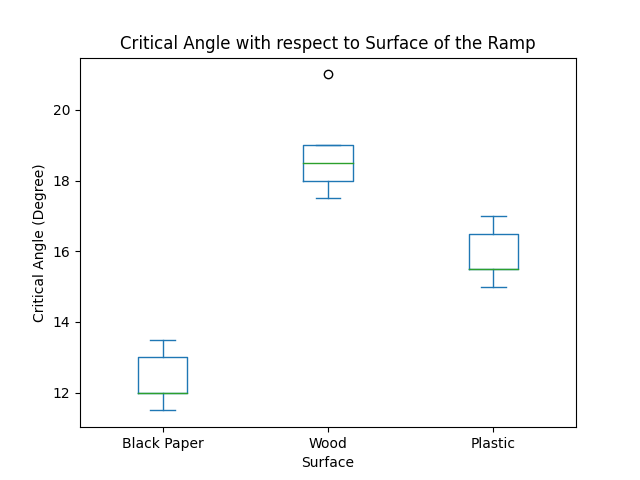
\includegraphics[width=100mm]{Static, Material.png}
    \label{graph:static-material}
\end{figure}

The collected data (and the graph) in general fits the expectation, since when varying the surface materials, the corresponding friction would also change accordingly, causing the critical angle (indicating the gravitational force's forward component matches the static friction) to vary based on materials.

\pagebreak

\subsection{Experiment for Static Friction with Varying Mass}
Here, the surface of the ramp is fixed as Paper.
\begin{table}[h!]
\centering
\begin{tabular}{c||c|c|c}
\toprule
\diagbox[width=3cm,height=1cm]{\textbf{Trial}}{\textbf{Mass (kg)}} & \textbf{0.292} & \textbf{0.493} & \textbf{0.577} \\
\midrule
1 & 11.000   & 10.500 & 10.500 \\
\hline
2 & 11.500 & 11.000   & 10.500 \\
\hline
3 & 11.000   & 10.500 & 10.000   \\
\hline
4 & 10.500 & 10.500 & 11.000   \\
\hline
5 & 10.500 & 10.000   & 11.000   \\
\midrule
\textbf{Average} & 10.900 & 10.500 & 10.600\\
\hline
\textbf{SD} & 0.418 & 0.354 & 0.418\\
\bottomrule
\end{tabular}
\caption{Critical Angle for Different Masses (Unit: Degree $ ^\circ$)}
\label{tab:static-mass}
\end{table}
\begin{figure}[h!]
    \centering
    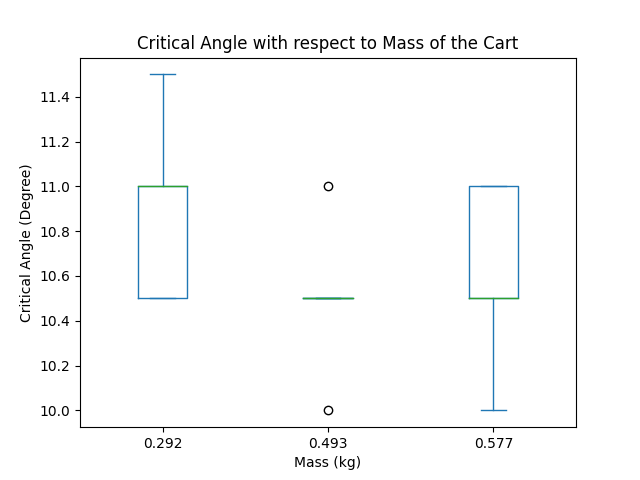
\includegraphics[width=100mm]{Static, Mass.png}
    \label{graph:static-mass}
\end{figure}

The collected data and the graph in general are as expected, since when scaling the mass accordingly, the porportionality between the normal force and the gravitational force's forward component stay the same (or, their ratio, which is proportional to the coefficient of static friction, is independent from mass). Then, the critical angle (indicating that grivational force's forward component and the static friction is equal), is also expected to be independent from mass, due to the same proportionality between friction and normal force, or it's not expected to see explicit change of critical angle when varying mass.

\pagebreak

\subsection{Experiment for Kinetic Friction}
Here, the surface of the ramp is fixed as Paper, and the mass of the cart is fixed as $0.292$ kg. Which, the cart always travel a distance of $0.275$ m.
\begin{table}[h!]
\centering

\begin{tabular}{c|| c| c| c}
\toprule
\diagbox[width=3cm,height=1cm]{\textbf{Trial}}{\textbf{Angle ($ ^\circ$)}} & \textbf{15°} & \textbf{17.5°} & \textbf{20°} \\
\midrule
1 & 0.960 & 0.790 & 0.710 \\
\hline
2 & 0.980 & 0.830 & 0.660 \\
\hline
3 & 1.060 & 0.790 & 0.660 \\
\hline
4 & 1.040 & 0.840 & 0.780 \\
\hline
5 & 0.990 & 0.830 & 0.630 \\
\midrule
\textbf{Average} & 1.006 & 0.816 & 0.688\\
\hline
\textbf{SD} & 0.042 & 0.024 & 0.059\\
\bottomrule
\end{tabular}
\caption{Object's Traveling Time for Different Angles (Unit: Second s)}
\label{tab:kinetic}
\end{table}
\begin{figure}[h!]
    \centering
    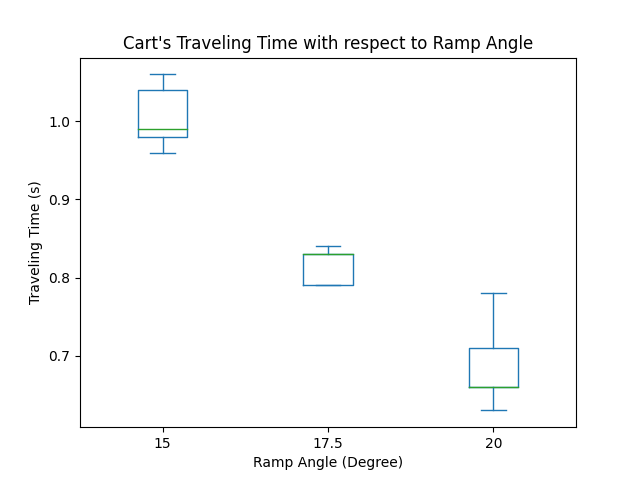
\includegraphics[width=100mm]{Kinetic, Angle.png}
    \label{graph:kinetic}
\end{figure}

The collected data and the graph in general are as expected, since when increasing the angle of the ramp, the gravitational force has a larger forward component. Also, since kinetic friction is only proportional to the normal force, while normal force decreases when ramp angle increases. Then, the total acceleration directed forward is expected to increase when ramp angle increases, which corresponds to a shorter traveling time for a fixed distance.

\pagebreak

\section{Data Analysis}
For this section, we'll need propogation of uncertainty through functions: Given a differentiable function $f:U \rightarrow \RR$ where $U \subseteq \RR^n$ with coordinates $(x_1,...,x_n)$, with a finite set of data labeled as $J$, then the Propogation of Uncertainty through $f$ is provided as:
\begin{align}
    \sigma_f := \sqrt{\sum_{i=1}^n \left(\frac{\partial f}{\partial x_i}\sigma_{x_i}\right)^2}
\end{align}

Then, for each of the section below, we'll calculate the corresponding coefficient of friction, and analyze its uncertainty using equation (1).

\subsection{Experiment for Static Friction with Varying Surface}
Recall from \textbf{Section 1} that for static friction, the coefficient of static friction $\mu_s =\tan(\theta)$ when given the critical angle $\theta$, which $\frac{d\mu_s}{d\theta}=\sec^2(\theta)$. Hence, based on data in Table \ref{tab:static-material}, the coefficients are provided as follow:

\begin{table}[h!]
\centering
\begin{tabular}{c|| c|c |c}
\toprule
\diagbox[width=3cm,height=1cm]{\textbf{Trial}}{\textbf{Surface}} & \textbf{Black Paper} & \textbf{Wood} & \textbf{Plastic} \\
\midrule
1 & 0.231 & 0.325 & 0.306 \\
\hline
2 & 0.240 & 0.344& 0.2678 \\
\hline
3 & 0.213 & 0.335 & 0.277 \\
\hline
4 & 0.213 & 0.384 & 0.296 \\
\hline
5 & 0.203 & 0.315 & 0.277 \\
\midrule
\textbf{Average} & 0.220 & 0.341 & 0.285\\
\hline
\textbf{Propogation of Uncertainty} & 0.862 & 1.507 & 0.888\\
\bottomrule
\end{tabular}
\caption{Coefficient of Static Friction for different Surfaces}
\label{tab:static-material-coe}
\end{table}
Using Propogation of Uncertainty in comparison to Standard Deviation (regular uncertainty), the uncertainty for the coefficient of static friction is relatively high compared to its average, indicating the collected data is not as valid (when using Propogation of Uncertainty as indicator of variance in the data). Nevetheless, one can still observe that the coefficient of static friction varies when changing the surface material of the ramp, one can still conclude that such coefficient has a decent confidence of being dependent to the surface of the ramp (if considering only the data).

\pagebreak

\subsection{Experiment for Static Friction with Varying Mass}
In this section, the calculation of coefficient of static friction $\mu_s$ is the same from the previoius section. Which, based on data in Table \ref{tab:static-mass}, the coefficients are provided as follow:
\begin{table}[h!]
\centering
\begin{tabular}{c ||c |c |c}
\toprule
\diagbox[width=3cm,height=1cm]{\textbf{Trial}}{\textbf{Mass (kg)}} & \textbf{ 0.292} & \textbf{0.493} & \textbf{0.577} \\
\midrule
1 & 0.194 & 0.185 & 0.185 \\
\hline
2 & 0.203 & 0.194 & 0.185 \\
\hline
3 & 0.194 & 0.185 & 0.176 \\
\hline
4 & 0.185 & 0.185 & 0.194 \\
\hline
5 & 0.185 & 0.176 & 0.194 \\
\midrule
\textbf{Average} & 0.193 & 0.185 & 0187\\
\hline
\textbf{Propogation of Uncertainty} & 0.434 & 0.366 & 0.433\\
\bottomrule
\end{tabular}
\caption{Coefficient of Static Friction for different Masses}
\label{tab:static-mass-coe}
\end{table}

In comparison to the previous experiment, in this section every collection of data of a manipulated variable corresponds to a relatively low Propogation of Uncertainty, yet such uncertainty is still relatively high compared to the calculated average, showing that this experiment still is not as valid for representing the coefficient of the model (when using Propogation of Uncertainty as indicator). Yet, based on the observation on the calculated data, one can still observe that the derived coefficients for each variable still has similar average value, which there is still a decent confidence to believe that mass change is not providing significant effect on the coefficient of static friction, in comparison to the surface material of the ramp (since in this experiment the surface is fixed).

\hfil

\subsection{Experiment for Kinetic Friction}
For kinetic friction, recall from kinematics that when starting at rest and under constant acceleration, the traveling distance $l=\frac{1}{2}at^2$, where $a$ is the total acceleration forward and $t$ is the traveling time. Hence, under the assumption of constant acceleration, total acceleration $a=\frac{2l}{t^2}$.

Also, with fixed ramp angle $\theta$, the forward acceleration caused by gravitational force is $g \sin(\theta)$, if let $a_f$ be the acceleration caused by friction (in backward direction), then $a = g\sin(\theta)-a_f$, hence $a_f = g\sin(\theta)-a=g\sin(\theta)-\frac{2l}{t^2}$. So, with mass $m$ the kinetic friction is $F_f=m a_f$.

Finally, given normal force $N=mg\cos(\theta)$, the coefficient of kinetic friction is given by $\mu_k=\frac{F_f}{N} = \frac{a_f}{g\cos(\theta)}=\tan(\theta)-\frac{2l}{g\cos(\theta)t^2}$. With time being the variable, $\frac{d\mu_k}{dt} = \frac{4l}{g\cos(\theta)t^3}$.

In this experiment, $l=0.275$ m, while $\theta=15^\circ, 17.5^\circ, 20^\circ$, based on the data in Table \ref{tab:kinetic}, the coefficients are provided as follow:

\pagebreak
\begin{table}[h!]
\centering
\caption{Calculated Values for Different Angles (Rounded to 3 Decimal Places)}
\begin{tabular}{c|| c| c| c}
\toprule
\diagbox[width=3cm,height=1cm]{\textbf{Trial}}{\textbf{Angle ($ ^\circ$)}} & \textbf{15} & \textbf{17.5} & \textbf{20} \\
\midrule
1 & 0.205 & 0.221 & 0.246 \\
\hline
2 & 0.207 & 0.230 & 0.227 \\
\hline
3 & 0.216 & 0.221 & 0.227 \\
\hline
4 & 0.214 & 0.232 & 0.266 \\
\hline
5 & 0.209 & 0.230 & 0.214 \\
\midrule
\textbf{Average} & 0.210 & 0.227 & 0.236 \\
\hline
\textbf{Propagation of Uncertainty} & 0.005 & 0.005 & 0.022 \\
\bottomrule
\end{tabular}
\end{table}

The Uncertainty of Propogation in this section are all small in comparison to the average coefficient of kinetic friction, showing there is a high validity the average can represent the actual coefficient for this experiment. One can observe that the average value of coefficient doesn't have siginicant changes when varying the ramp angle. And, from Table \ref{tab:static-mass}, one can conclude that the angle used in the experiment has a high confidence being higher than the calculated critical angle, which has average of $10.900, 10.500, 10.600$ degree (when fixing the surface material as paper). Hence, one can conclude that when the ramp angle is higher than the critical angle (when the gravitational force's forward component dominates the motion), coefficient of kinetic energy has a high confidence of beinng independent from the ramp angle.

\hfil

\section{Error Analysis}
Some potential error in this experiment (besides human mistakes and uncertainty caused by human's measurement limit) include:
\begin{itemize}
    \item The Effect of air resistance (which potentially provides unexpected external force in the experiment).
    \item The surface material having inconsistent property (causing coefficient of friction to vary across the surface).
\end{itemize}

\section{Conclusion}
In this experiment, when performing the two experiments for static friction, there are relatively low validity that the coefficients derived from the collected data can represent the actual coefficient of static friction due to a relatively high Propogation of Uncertainty. From the data itself however there is a certain confidence one can conclude that surface material is highly affecting the coefficient of static friction, while mass provides low effect on the coefficient.

For the experiment of kinetic friction, there is a relatively high validity that the coefficients derived from the collected data can represent the actual coefficient of kinetic friction, due to a relatively low Propogation of Uncertainty. And, since the average coefficient of kinetic friction across the three different ramp angle are close to each other, hence one can conclude that coefficient of kinetic friction has a high confidence of being independent from the ramp angle.

\newpage

\end{document}